\documentclass[12pt]{article}

\usepackage{hyperref}
\usepackage{float, graphicx}
\usepackage[margin=2.5cm]{geometry}
\usepackage{amsmath, amssymb}

\begin{document}

\begin{titlepage}
    \begin{center}
        ~\\[2.0cm]

        \textsc{\LARGE McGill University}\\[1.5cm]

        \textsc{\Large Undergraduate Research Course in Human Genetics (HGEN 396)}\\[1.0cm]

        {\huge \bfseries Difference Map Optimizer \\ a new method for the unconstrained global optimization of multivariate scalar functions}

        ~\\[2.0cm]

        \emph{By}\\
        Jacob Thomas Errington (260636023)\\[1.0cm]

        \emph{Presented to}\\
        Dr. Simon Gravel

        \vfill

        \today
    \end{center}
\end{titlepage}

\begin{abstract}

Global optimizers are valuable tools in many contexts:
whereas some intractable problems are frequently approximated, as exact
solutions may be too costly to compute, certain problems have no analytic
solutions.
We propose a deterministic metaheuristic for the global optimization
problem, using an iteration scheme based on local searches combined with an
internal estimate of the objective function's global minimum.
Our method is empirically compared to existing state-of-the-art methods on
a handful of difficult functions and its perceived strengths and weaknesses
are outlined.
We conclude that although our method is comparable in effectiveness to the
state-of-the-art as an out-of-the-box tool requiring practically no
tweaking, it is outperformed by contemporary methods that are first
adjusted by the practitioner to suit the problem at hand.

\end{abstract}

\section{Introduction}

Metaheuristics are useful due to their wide applicability, finding use in
problems where the function to optimize is noisy, discrete, or
discontinuous.

As such, the very broad problem with which we concern ourselves is
$$
\min_{x \in \mathbb{R}^n} f(x)
$$
where $f : \mathbb{R}^n \to \mathbb{R}$,
i.e. we wish to find $x^* \in \mathbb{R}^n$
such that $f(x^*) \leq f(x)$ for all $x \in \mathbb{R}^n$.

\emph{Simulated Annealing}\cite{kirkpatrick1983} is perhaps one of the most
well-known and most extensively studied metaheuristics.
The intuition for it comes from the \emph{annealing} procedure in
metallurgy, in which a metal is brought to a high temperature before being
gradually cooled.
The greater energy of the high-temperature particles allows for many
potentially unstable configurations to be tried, in the hopes that as the
metal is slowly cooled, energy-minimizing arrangements will be found.
Thus, the annealing's \emph{cooling schedule} is important in avoiding
local minima, as a slower one would allow the particles more time to
stochastically try many different arrangements, whereas a faster one would
offer them fewer such chances.

A higher temperature value results in more liberal acceptance of new,
higher-energy coordinates.
Hence the search space is broadly explored while the temperature is high.
As the temperature decreases, the acceptance of new coordinates becomes
more selective; at a temperature of zero, only coordinates strictly better
than the current position will be accepted.

The Simulated Annealing algorithm thus consists of two essential steps:
\begin{enumerate}
    \item random perturbation of the coordinates;
    \item accept or reject the new coordinates based on the current
        temperature.
\end{enumerate}

\emph{Basin Hopping}\cite{wales1997} is a popular variation on Simulated
Annealing.
Simply put, a local minimization is performed prior to the accept-or-reject
step, and the accept-or-reject is performed based on the results of that
local search.
Of course, this method is available only to functions in which local
searches are possible.
Basin Hopping is thus less robust, but seems to provide better performance
on smooth functions with many local minima.

\emph{Differential Evolution}\cite{storn1997} is a metaheuristic based on
\emph{recombination} and \emph{selection}, processes in genetics whereby
two chromosomes exchange pieces of information and whereby unfit
individuals are removed from the population, respectively.
In the context of optimization, the chromosomes are candidate solution
vectors, and the exchanged pieces of information roughly correspond to
entries of those vectors. As for selection, candidate solutions with
smaller function values are favoured over those high higher function
values.

Three control parameters greatly affect the effectiveness of Differential
Evolution and must be chosen by the practitioner\cite{storn1997}: the
population size, the differential weight, and the crossover probability.
In fact, the choice of these parameters has been the topic of
meta-optimization\cite{pedersen2010}.

The \emph{Simplex Method}\cite{nelder1965}, frequently called the
\emph{Nelder-Mead} method after its creators (and to avoid confusion with a
similarly named method for linear programming), is a much older
minimization strategy. Although originally conceived as a local
minimization technique, it can be applied to global minimization as well.

If the dimension of the search space is $n$, then $n+1$ points are first
chosen to form a simplex in the space. The intuition for this method is to
let the simplex tumble down the local minimum, expanding and contracting as
twists and turns are encountered in the function. In particular, on each
iteration, the vertex with the worst score (highest function value) is
replaced by reflecting it through the centroid of the simplex. The simplex
is expanded or contracted according to the quality of the reflection.

As such, a number of parameters are again to be chosen by the practitioner,
namely the ratios to use when reflecting, expanding, and contracting the
simplex.

\section{Objective}

In the above survey of existing methods, each optimization technique
requires a number of parameters that must be chosen \emph{a priori}. On the
one hand, these methods are very general thanks to the parameters that can
be tweaked to adapt them to many different problems. On the other hand,
this can make them difficult to use when it is not clear how the parameters
should be chosen.

With that in mind, it is our goal to design an optimization technique
requiring as little configuration as possible; our method should work
\emph{out-of-the-box} on a variety of problems. Furthermore, it is desired
that our method outperform Simulated Annealing.

The rationale for singling out Simulated Annealing, is that it is perhaps
the most extensively studied metaheuristic, and is perhaps the most
general, having been specialized in many applications. Equally, we would
prefer our method to have a certain potential to be specialized further.


\section{Methods}

\subsection{Difference Map Optimizer}
The method we propose, called the \emph{Difference Map Optimizer} (DMO), is
based on the \emph{Difference Map}\cite{elser2007}, a constraint
satisfaction algorithm.
Despite being an iterative projection technique, which have a reputation
for becoming trapped in local minima, the Difference Map can avoid
stagnation in a local minimum precisely by using a difference of the two
elementary projections of its current iterate onto the two constraints to
be satisfied. As such, the iterate is kept distinct from its projections
onto the constraints.

DMO is an iterative metaheuristic that uses local searches on each
iteration to gradually build up a landscape of the search space.
Furthermore, rather than have the iterate follow the local search, the
results of the local searches are kept distinct from the iterate.
As a mechanism for adapting to different functions, DMO maintains an
internal estimate of the global minimum, denoted $t$, which affects the
sizes of the steps taken by the iterate. By analogy with the Difference Map
from which we derive our intuition for DMO, the projection operator is the
local search.

First, two starting points $x_0$ and $x_1$ are selected from the search
space.
A local minimization is performed on $x_0$ to find $x_0^*$ and the
initial value for the target is computed as
$t := f(x_0^*) - s (f(x_0) - f(x_0^*))$,
where $s$ is a scaling factor that controls the overall greediness of the
algorithm.
The point $x_1$ is taken as the initial position of the iterate. Our
experiments showed that $x_0$ and $x_1$ should be chosen to be close to
each other, yet ideally in different attractors.
The points $x_0^*$ and $x_0$ are then added to a running list $M$ of
minimizers discovered so far.

On each iteration starting from the position of the iterate $x_i$, a local
minimizer $x_i^*$ is found by traditional local optimization techniques.
If $f(x_i^*)$ is less than the current estimate, then the estimate is
recalculated as before, but using $f(x_i^*)$ and $\min_{x \in M} f(x)$.
Then, the point $x_{near} \in M$ with the least distance to $x_i^*$ is
selected.
From $x_{near}$, the step to take is calculated.
\begin{equation}
    \Delta x_i =
        \frac{t - f(x_i^*)}{f(x_i^*) - f(x_{near})} (x_i^* - x_{near})
    \label{eqn:dx}
\end{equation}

The next position of the iterate is obtained by applying the step
$\Delta x_i$.
$$
    x_{i+1} = x_i + \Delta x_i
$$

Figure \ref{fig:iteration} provides a visualization of the iteration
procedure.

Note that if the quantity $f(x_i^*) - f(x_{near}$ is close to zero, i.e.
$|f(x_i^*) - f(x_{near})| < tol$ where $tol$ is a predetermined tolerance
for numerically distinguishing reals, then that quantity should be
replaced with $tol$.
Under these circumstances, which arise when the local landscape of the
function appears very flat, the iterate is to be moved infinitely far away.
Of course this is not possible, so a numerical approximation is chosen
instead.

Finally, the point $x_0^*$ is added to the set of discovered minimizers
$M$, and the target value $t$ is updated.

Many update strategies are possible, but our experiments showed that merely
recalculating the target, as above, every $r$ iterations using the two
smallest values $f(x)$ for $x \in M$ produced acceptable estimates of the
global minimum.

\begin{figure}[H]
    \begin{center}
        \includegraphics[width=0.8\textwidth]{../figures/iteratingnew.png}
        \caption{An example iteration of the Difference Map Optimizer.
            The orange points are, from left to right, the iterate $x_i$
            and its associated local minimum $x_i^*$. The blue point is the
            nearest previously discovered local minimum $x_{near}$.
            The orange and blue lines represent the function values of
            these two local minimizers, and the red line represents the
            current target value. In this example, the iterate will be
            moved in the negative $x$ direction.}
        \label{fig:iteration}
    \end{center}
\end{figure}


\subsection{Benchmarking}

Wolfram \emph{Mathematica} provides implementations of several of the
optimization methods presented earlier.
In particular, Simulated Annealing, Differential Evolution, and Nelder-Mead
are implemented.
As such, \emph{Mathematica} is used as our primary environment for testing
DMO.
All tests are conducted with version $10.0$ of \emph{Mathematica} on an
Apple iMac (late 2013) running Ubuntu, with a $3.1$~GHz Intel i7 processor
and $16$~GB of $1600$~MHz DDR3 RAM.
Our reference implementation of DMO can be found online at
\url{https://github.com/djeik/dm_optimizer}.

First, since our primary goal is to design an out-of-the-box algorithm,
we compare DMO to each of the \emph{Mathematica} optimizers with as little
tweaking as possible.

Second, a minor tweak to the \emph{Mathematica} optimizers is applied. This
will allow a comparison between DMO, which is requires to such tweaking,
and solvers that are effectively being advantaged by this extra information
concerning the problem space.

The tweak in question is essentially a \emph{bracketing} of the search
space. In some applications it is possible to bracket the optimum, but in
others, it is not. Hence, we believe that it is worthwhile to explore both
these avenues.

In order to compare the solvers in the fairest way possible, each solver is
run such that the average number of function evaluations per run is
approximately $20~000$.

As the connection between the maximum number of allowed interations and the
number of function evaluations is rather unclear for the \emph{Mathematica}
methods, a particular proportion was used to estimate how many iterations
each solver should be run for in order to obtain the desired number of
function evaluations.
Specifically, each solver is run for some small number of iterations,
\emph{e.g.} $5$, and the number of function evaluations is counted.
A ratio of function evaluations per iteration is computed and scaled to
match the desired $20~000$ iterations.

The reason we choose to average over a small number of iterations rather
than a larger one is due to an oddity in \emph{Mathematica}.
In the region of small iteration counts, the number of function evaluations
appears to scale roughly linearly, but in higher ranges this appears to be
no longer true.
For instance, some of our tests showed that Simulated Annealing would seem
to stall around $750$ function evaluations, no matter how high the number
of iterations was set.

Stalls in the \emph{Mathematica} optimizers are dealt with by a random
restart process: if the solver generates an insufficient number of function
evaluations, then the solver is restarted with a different random seed.
It is of note that a new starting point for the solver is not picked, as
could improve the odds of the solver landing in the global minimum at the
first iteration, which would unfairly advantage the randomly restarting
solvers. Thus, by changing only the seed for the random number generator,
it is only the trajectory of the solver that is affected.

\pagebreak

\section{Results}
\begin{figure}[H]
    \begin{center}
        {\large {\bfseries Solutions found per solver per function}\\
        for unbracketed \emph{Mathematica} solvers}

        \includegraphics[width=0.45\textwidth]{../figures/ackley-fun-bad.pdf}
        \includegraphics[width=0.45\textwidth]{../figures/griewank-fun-bad.pdf}
        \includegraphics[width=0.45\textwidth]{../figures/rosenbrock-fun-bad.pdf}
        \includegraphics[width=0.45\textwidth]{../figures/f1-fun-bad.pdf}
        \includegraphics[width=0.45\textwidth]{../figures/h4-fun-bad.pdf}

        \caption{
            A distribution chart of the global minimum found for each
            solver, for each tested objective function. For each solver,
            $25$~runs were performed, with the iteration count for each
            solver adjusted to perform a total of approximately $20~000$
            function evaluations. The \emph{Mathematica} solvers that
            generated this dataset were \emph{not} given bracketing
            information concerning the objective function.
        }
        \label{fig:bad-data}
    \end{center}
\end{figure}

From figure \ref{fig:bad-data}, we can see that DMO performs comparably to
Simulated Annealing in the Ackley, Griewank, F1 functions, but is
outperformed in the Rosenbrock and H4 functions.

\begin{figure}[H]
    \begin{center}
        {\large {\bfseries Exploration patterns of \emph{Mathematica}'s solvers}\\
        for both unbracketed and bracketed configurations}
        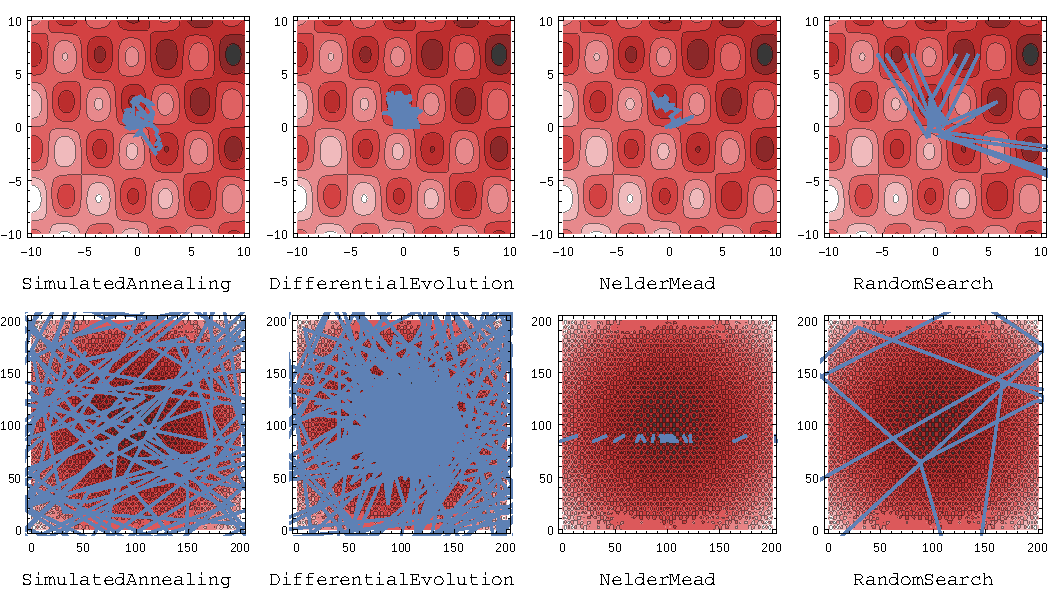
\includegraphics[width=\textwidth]{../figures/mma-compare-brackets.pdf}
        \caption{The exploration patterns of the built-in
        \emph{Mathematica} optimizers. The explorations on the top row are
            generated by using the default sampling range in the search
            space, $-1 < x_i < 1$ for $1 \leq i \leq n$ where $n$ is the
            dimension of the search space. On the bottom row, the sampling
            range is much larger. The objective function used in the above
            is the \emph{Griewank} function, for which the suggested
            evaluation range is $-600 < x_i < 600$ for each
            $x_i$\cite{griewank1981}. The change in scale between the plots
            in the top and bottom rows is large. % TODO this is lame.
        }
        \label{fig:exploration}
    \end{center}
\end{figure}

Figure \ref{fig:exploration} demonstrates the crucial difference made by
endowing the solvers with the bracketing information concerning the search
space. The search space is explored far more effectively, as one would
expect. We suspect that this information is used by Simulated Annealing to
determine by how much it should perturb its coordinate vector. Likewise, we
believe that Differential Evolution can create its population of candidate
vectors in a more principled and spread out manner thanks to this
additional information.

\begin{figure}[H]
    \begin{center}
        {\large {\bfseries Comparing exploration patterns of DMO and Simulated Annealing}\\
        with both bracketed and unbracketed Simulated Annealing runs}
        \includegraphics[width=0.8\textwidth]{../figures/ackley-dm-sa-bracketing-compare.pdf}

        \caption{
            A comparison of the exploration patterns of DMO and Simulated
            Annealing on the Ackley function. Without bracketing
            information, Simulated Annealing (orange) performs very badly,
            and hardly explores the search space. Given this additional
            bracketing information, its exploration (blue) is similar to
            DMO's (green).
        }
        \label{fig:dm-sa-bracket-exploration}
    \end{center}
\end{figure}


With this additional information, the mathematica solvers do outperform DMO
in all cases, as seen in figure \ref{fig:good-data}.

\begin{figure}[H]
    \begin{center}
        {\large {\bfseries Solutions found per solver per function}\\
        for bracketed \emph{Mathematica} solvers}

        \includegraphics[width=0.45\textwidth]{../figures/ackley-good.pdf}
        \includegraphics[width=0.45\textwidth]{../figures/griewank-good.pdf}
        \includegraphics[width=0.45\textwidth]{../figures/rosenbrock-good.pdf}
        \includegraphics[width=0.45\textwidth]{../figures/f1-good.pdf}
        \includegraphics[width=0.45\textwidth]{../figures/h4-good.pdf}

        \caption{
            A distribution chart of the global minimum found for each
            solver, for each tested objective function. For each solver,
            $25$~runs were performed, with the iteration count for each
            solver adjusted to perform a total of approximately $20~000$
            function evaluations. The \emph{Mathematica} solvers that
            generated this dataset were given bracketing information
            concerning the objective function.
        }
        \label{fig:good-data}
    \end{center}
\end{figure}

\pagebreak

\section{Conclusion}

We have presented Difference Map Optimizer, a metaheuristic for the global
optimization of scalar functions of several variables.
The intuition for it comes from the Difference Map, a constraint satisfaction
algorithm of surprising efficiency and simplicity.

The essential property of DMO is that it requires hardly no configuration, and
is able to traverse the search space in a principled manner without becoming
trapped in local minima.
Furthermore, unlike contemporary methods that seek to emulate stochastic
processes as effective optimization algorithms, DMO is deterministic.

In problems for which information concerning the search space is very limited,
DMO may show a lot of promise.
However, in problems where information about the search space is available,
other methods are at this time still more appropriate.

With that in mind, there is still considerable room for improvement in DMO. For
instance, the outliers in figures \ref{fig:good-data} and \ref{fig:bad-data} in
the Rosenbrock function are perhaps the result of DMO having no intrinsic way
to ensure that its search converges, or stays within reasonable limits. Indeed,
that is in some sense a strength of DMO: it has no notion of what is reasonable
beyond its internal estimate of the global minimum. Moreover, whereas Simulated
Annealing progressively becomes more conservative in its choices as time goes
by, DMO does not even keep track of how much time has elapsed beyond how many
local minima have been discovered thus far.

Overall, the Difference Map Optimizer is interesting due to these perceived
strengths and its sheer novelty as an optimization technique. Although it is
not presently ready for use in production environments, the different
approaches to improving it are clear.

\pagebreak

\bibliographystyle{plain}
\bibliography{dm}

\end{document}
